% Rúbrica del curso: máximo 20 páginas, 1 columna, tamaño de fuente 12
\documentclass[12pt,a4paper]{article}

% ---------- Idioma y codificación ----------
\usepackage[utf8]{inputenc}
\usepackage[T1]{fontenc}
\usepackage[spanish]{babel}
\decimalpoint % todas las cifras del reporte usan punto decimal, no coma

% ---------- Página ----------
\usepackage[margin=2.0cm]{geometry}
\setlength{\emergencystretch}{3em}
\sloppy

% ---------- Tablas ----------
\usepackage{booktabs}
\usepackage{tabularx}
\usepackage{array}
\usepackage{longtable}
\usepackage{multirow}

% ---------- Figuras ----------
\usepackage{graphicx}
\usepackage{float}

% ---------- Código ----------
\usepackage{listings}
\usepackage{xcolor}

\lstdefinestyle{sql}{
  basicstyle=\ttfamily\small,
  breaklines=true,
  frame=single,
  columns=fullflexible,
  backgroundcolor=\color{gray!8},
  keywordstyle=\color{blue!60!black}\bfseries,
  commentstyle=\color{green!40!black},
  showstringspaces=false
}
\lstset{style=sql}

% ---------- Cuadros de advertencia (secciones pendientes) ----------
\usepackage{tcolorbox}
\tcbuselibrary{skins,breakable}
\newtcolorbox{pendiente}{
  colback=yellow!10,
  colframe=yellow!50!black,
  boxrule=0.5pt,
  breakable,
  title={Sección pendiente}
}

% ---------- Diagramas TikZ ----------
\usepackage{tikz}
\usetikzlibrary{shapes.geometric, arrows.meta, positioning}

% ---------- Símbolos y math ----------
\usepackage{amsmath}
\usepackage{amssymb}

% ---------- Hipervínculos (al final del preámbulo) ----------
\usepackage[colorlinks=true, linkcolor=blue!50!black, urlcolor=blue!50!black, citecolor=blue!50!black]{hyperref}

\begin{document}

% ---------- Portada (armada a mano para controlar el tamaño de fuente) ----------
\begin{titlepage}
\begin{center}
\vspace*{2cm}
{\LARGE Proyecto Big Data G5: Uso de Bicicletas (Londres)} \\[0.5em]
{\large Módulo: Ingeniería y Analítica de Grandes Cantidades de Datos}

\vspace{1.5cm}
{\normalsize Grupo 5}

\vspace{0.8cm}
{\normalsize
\begin{tabular}{cc}
Cevallos Vinces Nahin Jussephe & Sanchez Guzman Annabella Noelia \\[0.5em]
Martha Maritza Duran Navarrete & Suarez Aspiazu Jesus David \\[0.5em]
Martin Pimentel Isabella Ivonne & Zurita Guerrero Angelo Saul \\[0.5em]
\multicolumn{2}{c}{Munizaga Torres Juan Andres}
\end{tabular}
}

\vspace{1.5cm}
{\normalsize 18 de septiembre de 2026}
\end{center}
\end{titlepage}

\newpage
\tableofcontents
\newpage

\section{Resumen ejecutivo}

Tres motores de datos con arquitecturas distintas responden las mismas tres preguntas analíticas sobre 38.2 millones de viajes del sistema público de bicicletas de Londres, medidos en tres computadoras y en dos etapas: leyendo el CSV original y leyendo un artefacto pre-procesado.

Se compararon \textbf{Pandas} (DataFrame en memoria, columnar sobre NumPy, mono-hilo), \textbf{DuckDB} (motor OLAP columnar embebido, vectorizado y multi-hilo) y \textbf{SQLite} (motor OLTP embebido, orientado a filas). Cada combinación de versión, herramienta y pregunta se ejecutó de forma independiente, cargando el archivo desde cero, con un presupuesto de 10 minutos por ejecución.

Tres hallazgos sostienen el trabajo:

\begin{enumerate}
  \item \textbf{El umbral de Big Data no es una cifra de filas ni de gigabytes.} La versión XL resultó imposible en una máquina de 15.7 GB de RAM y perfectamente manejable en una de 8 GB. Big Data es una propiedad de la relación entre datos, representación y hardware.
  \item \textbf{Cambiar la representación mueve ese umbral sin tocar el hardware.} El equipo que falló leyendo el CSV de 4.7 GB completó la misma carga de trabajo en 6.0 segundos sobre el artefacto optimizado.
  \item \textbf{La arquitectura de almacenamiento pesa más que las especificaciones.} DuckDB resolvió el dataset completo en 2.7 segundos en la máquina de menor RAM del grupo, mientras SQLite necesitaba varios minutos en la de 40 GB. Un índice B-tree no convierte un motor OLTP en columnar.
\end{enumerate}

\section{Dataset y versiones}
\label{sec:dataset}

La fuente es el conjunto \href{https://www.kaggle.com/datasets/ajohrn/bikeshare-usage-in-london-and-taipei-network}{Bikeshare usage in London and Taipei} de Kaggle. \textbf{El alcance de este trabajo es únicamente la red de Londres}; los datos de Taipéi quedan fuera por decisión de equipo.

Se trabajó con el histórico de viajes en cinco versiones de tamaño creciente, más \texttt{london\_stations.csv}, un catálogo de 802 estaciones con nombre, latitud y longitud.

\begin{table}[htbp]
\centering
\caption{Versiones disponibles del dataset}
\label{tab:versiones}
\begin{tabular}{lrrrr}
\toprule
Versión & Archivo & Tamaño (GB) & Filas & Factor vs. XS \\
\midrule
XS & \texttt{london\_xs.csv} & 0.049 & 398,075 & $1.0\times$ \\
S  & \texttt{london\_s.csv}  & 0.488 & 3,972,436 & $10.0\times$ \\
M  & \texttt{london\_m.csv}  & 1.181 & 9,590,698 & $24.1\times$ \\
L  & \texttt{london\_l.csv}  & 2.363 & 19,148,881 & $48.1\times$ \\
XL & \texttt{london.csv}     & 4.725 & 38,215,560 & $96.0\times$ \\
\bottomrule
\end{tabular}
\end{table}

El esquema tiene nueve columnas: \texttt{rental\_id}, \texttt{duration}, \texttt{bike\_id}, \texttt{start\_rental\_date\_time}, \texttt{end\_rental\_date\_time}, \texttt{start\_station\_id}, \texttt{start\_station\_name}, \texttt{end\_station\_id}, \texttt{end\_station\_name}.

La exploración inicial, hecha con DuckDB en streaming para no cargar los archivos grandes en memoria, detectó cuatro problemas de calidad:

\begin{itemize}
  \item \texttt{end\_station\_id} tiene nulos, que corresponden a viajes sin devolución registrada. Se excluyen de las llegadas y de los pares origen-destino.
  \item \texttt{duration} contiene ceros y valores extremos de varios días. No intervienen en las tres preguntas, pero se documentan.
  \item \texttt{start\_station\_id} es entero mientras \texttt{end\_station\_id} se infiere como \texttt{DOUBLE} por causa de los nulos. Hay que castear explícitamente para que los identificadores comparen igual en las tres herramientas.
  \item El catálogo tiene 802 estaciones, pero Q2 y Q3 (Sección \ref{sec:respuestas}) reportan 808 identificadores de estación distintos, porque esa cifra sale directo de los \texttt{station\_id} que aparecen como origen o destino en los viajes, no del catálogo. Siete \texttt{station\_id} (391, 346, 304, 434, 241, 825, 823) no están en \texttt{london\_stations.csv}; la 391 por sí sola acumula 9,050 viajes. El join contra el catálogo es left join y las rellena con la etiqueta \texttt{(estación N)}, así que no rompen Q2 ni Q3, pero al no tener latitud ni longitud quedan fuera de la Figura \ref{fig:q2-mapa} (la estación 391 incluida), y su nombre se pierde de forma irrecuperable en la proyección a 4 columnas de la Fase 3 (Sección \ref{sec:fase3-diagnostico}).
\end{itemize}

El rango de fechas cambia con la versión: las versiones chicas cubren pocas semanas y las grandes cubren más meses. Eso altera la interpretación de la estacionalidad, no el método.

\section{Metodología}

\subsection{Las tres preguntas}

\begin{table}[htbp]
\centering
\caption{Preguntas analíticas del proyecto}
\label{tab:preguntas}
\begin{tabularx}{\textwidth}{clX}
\toprule
\# & Pregunta & Salida \\
\midrule
Q1 & ¿Cómo varía la demanda de viajes por hora del día y día de la semana? & 168 combinaciones día $\times$ hora \\
Q2 & ¿Qué estaciones tienen mayor desequilibrio entre llegadas y salidas? & 808 estaciones con actividad \\
Q3 & ¿Existen rutas origen-destino que concentran gran parte del tráfico? & 510,672 rutas distintas \\
\bottomrule
\end{tabularx}
\end{table}

\subsection{Las tres herramientas}

\begin{table}[htbp]
\centering
\caption{Herramientas comparadas}
\label{tab:herramientas}
\begin{tabularx}{\textwidth}{lXX}
\toprule
Herramienta & Arquitectura & Por qué está en la comparación \\
\midrule
Pandas & DataFrame en memoria, columnar sobre NumPy, mono-hilo & Caso base: rápido mientras el dataset quepa en RAM \\
DuckDB & Motor OLAP columnar embebido, vectorizado y multi-hilo & Diseñado exactamente para este tipo de agregación \\
SQLite & Motor OLTP embebido, orientado a filas & Misma interfaz SQL, arquitectura de almacenamiento opuesta \\
\bottomrule
\end{tabularx}
\end{table}

SQLite es la tercera herramienta y aporta el contraste más informativo del trabajo: comparte el lenguaje con DuckDB pero no su modelo de almacenamiento, así que aísla el efecto de la arquitectura frente al del lenguaje de consulta.

\subsection{Protocolo de ejecución independiente}

Cada combinación de versión, herramienta y pregunta es una \textbf{ejecución independiente que arranca desde el archivo}: se carga desde cero y después se corre la consulta. El tiempo reportado es carga $+$ query, y ese es el número que se compara contra el límite de 10 minutos.

La razón es que SQLite no conserva el archivo cargado entre consultas, a diferencia de Pandas, que mantiene el DataFrame en RAM, y de DuckDB, que mantiene la tabla en memoria. Aplicar el mismo protocolo a las tres evita que alguna se beneficie de reutilizar una carga que otra tuvo que repetir.

Otras reglas que sostienen la honestidad de la medición:

\begin{itemize}
  \item La carga a SQLite \textbf{no usa Pandas}. Se lee el CSV en streaming con el módulo \texttt{csv} de la librería estándar y se inserta por lotes de 200,000 filas con \texttt{executemany}. Usar \texttt{df.to\_sql()} mediría a Pandas disfrazado de SQLite.
  \item DuckDB \textbf{materializa} la tabla con \texttt{CREATE TABLE ... AS SELECT}, en vez de leer el CSV de forma perezosa, para competir en igualdad de condiciones con \texttt{pd.read\_csv()}.
  \item La base SQLite se crea desde cero en cada ejecución y se borra al terminar.
  \item El pico de RAM se captura con un hilo que muestrea el proceso cada 50 ms. Medir solo antes y después perdería el pico transitorio que ocurre dentro de la lectura.
  \item Los días de la semana se normalizan a lunes $=0$ en las tres herramientas, porque cada motor los numera distinto.
\end{itemize}

\subsection{Validación cruzada}

Un benchmark solo vale si las tres herramientas responden lo mismo. Los resultados se comparan celda a celda contra Pandas como referencia, con tolerancia numérica en las columnas de porcentaje, y se verifica el cuadre aritmético: la suma de viajes de Q1 debe igualar el número de filas del archivo, y las llegadas de Q2 deben igualar el total de Q3. \textbf{Las tres herramientas produjeron resultados idénticos en todas las versiones que completaron.}

\section{Equipos de cómputo}

El barrido se corrió en tres máquinas con perfiles deliberadamente distintos. Esa diversidad es lo que permite responder dónde empieza a ser Big Data, porque la respuesta cambia con el equipo.

\begin{table}[htbp]
\centering
\small
\caption{Ficha técnica de los equipos utilizados}
\label{tab:equipos}
\begin{tabularx}{\textwidth}{lXXrrX}
\toprule
Equipo & Sistema & Procesador & Núcleos (físicos/lógicos) & RAM & Versiones corridas \\
\midrule
Pc\_Jesus  & macOS Darwin 27.0 (arm64) & Apple arm, 3.20 GHz & 8 / 8 & 8.0 GB & M, L, XL \\
Pc\_Martha & Windows 11 (AMD64) & Intel i7 gen 13, 1.70 GHz & 10 / 12 & 15.7 GB & XS, S, M, L, XL \\
Pc\_Nahin  & Windows 11 (AMD64) & Intel Core Ultra 9 185H, 2.30 GHz & 16 / 22 & 39.4 GB & M, L, XL \\
\bottomrule
\end{tabularx}
\end{table}

\subsection{Versiones de software}

Las versiones no son idénticas entre equipos. La diferencia es menor frente a las brechas de orden de magnitud que se observan, pero se declara por transparencia.

\begin{table}[htbp]
\centering
\caption{Versiones de software por equipo}
\label{tab:software}
\begin{tabular}{lccccc}
\toprule
Equipo & Python & pandas & duckdb & sqlite & numpy \\
\midrule
Pc\_Jesus  & 3.14.3  & 3.0.5 & 1.5.5 & 3.50.4 & 2.5.3 \\
Pc\_Martha & 3.12.10 & 3.0.2 & 1.5.5 & 3.49.1 & 2.4.4 \\
Pc\_Nahin  & 3.14.0  & 3.0.1 & 1.5.5 & 3.50.4 & 2.4.3 \\
\bottomrule
\end{tabular}
\end{table}

Las tres máquinas corren DuckDB 1.5.5, así que las diferencias de rendimiento entre ellas no se explican por la versión del motor analítico.

\section{Fase 2: Línea base}

De la versión S en adelante, DuckDB es entre 4 y 11 veces más rápido que Pandas y entre 17 y 30 veces más rápido que SQLite sobre el mismo CSV. El orden se mantiene en las tres máquinas y en todas las versiones.

\subsection{Tiempo total por herramienta y versión}

Suma de las tres preguntas, en segundos. Cada celda es carga $+$ query acumulado. El desglose por pregunta de cada equipo está en los archivos \texttt{benchmarks\_*.csv} del repositorio.

\begin{table}[htbp]
\centering
\small
\caption{Tiempo total (carga + query) por versión, equipo y herramienta}
\label{tab:fase2-tiempos}
\begin{tabular}{llrrr}
\toprule
Versión & Equipo & Pandas & DuckDB & SQLite \\
\midrule
XS & Pc\_Martha & 1.9   & 0.7   & 5.8 \\
S  & Pc\_Martha & 29.5  & 4.0   & 97.2 \\
M  & Pc\_Jesus  & 34.5  & 5.0   & 108.2 \\
M  & Pc\_Martha & 50.0  & 6.7   & 164.6 \\
M  & Pc\_Nahin  & 143.1 & 15.3  & 445.0 \\
L  & Pc\_Jesus  & 79.1  & 11.5  & 232.8 \\
L  & Pc\_Martha & 106.5 & 15.3  & 404.0 \\
L  & Pc\_Nahin  & 288.1 & 25.9  & 776.9 \\
XL & Pc\_Jesus  & 195.4 & 27.3  & 472.6 \\
XL & Pc\_Martha & falló & falló & falló \\
XL & Pc\_Nahin  & 501.4 & 122.3 & excedió \\
\bottomrule
\end{tabular}
\end{table}

\subsection{Por qué ese orden}

\textbf{DuckDB} almacena por columnas y ejecuta de forma vectorizada y multi-hilo. Para un \texttt{GROUP BY} lee únicamente las dos o tres columnas que necesita; el resto del ancho de fila nunca toca el disco ni la RAM.

\textbf{Pandas} también es columnar en memoria y vectorizado sobre NumPy, pero es mono-hilo y paga materializar las nueve columnas, incluidas las dos de texto con los nombres de estación, que son las más caras de parsear y las que más memoria ocupan.

\textbf{SQLite} está orientado a filas. Un \texttt{GROUP BY} recorre cada registro completo y parsea los timestamps con \texttt{strftime} fila por fila. Es el comportamiento esperado: SQLite está optimizado para OLTP, es decir, buscar e insertar pocas filas por clave, no para agregar decenas de millones.

\subsection{Dónde se va el tiempo}

El desglose entre carga y consulta es la observación que justifica toda la Fase 3. En la versión XL sobre Pc\_Jesus:

\begin{table}[htbp]
\centering
\caption{Desglose carga vs. query, versión XL, Pc\_Jesus}
\label{tab:fase2-desglose}
\begin{tabular}{llrrr}
\toprule
Herramienta & Pregunta & Carga (s) & Query (s) & \% en carga \\
\midrule
Pandas & Q1 & 56.7 & 2.7  & 95\% \\
Pandas & Q3 & 57.2 & 21.6 & 73\% \\
DuckDB & Q1 & 9.0  & 0.3  & 97\% \\
DuckDB & Q3 & 8.1  & 1.4  & 85\% \\
SQLite & Q1 & 99.8 & 28.6 & 78\% \\
SQLite & Q2 & 108.8& 82.6 & 57\% \\
\bottomrule
\end{tabular}
\end{table}

La carga domina en todos los casos. Y como el protocolo obliga a recargar el archivo en cada pregunta, ese costo se paga tres veces. \textbf{El formato de almacenamiento es, entonces, la palanca de optimización más rentable disponible.}

\begin{figure}[htbp]
  \centering
  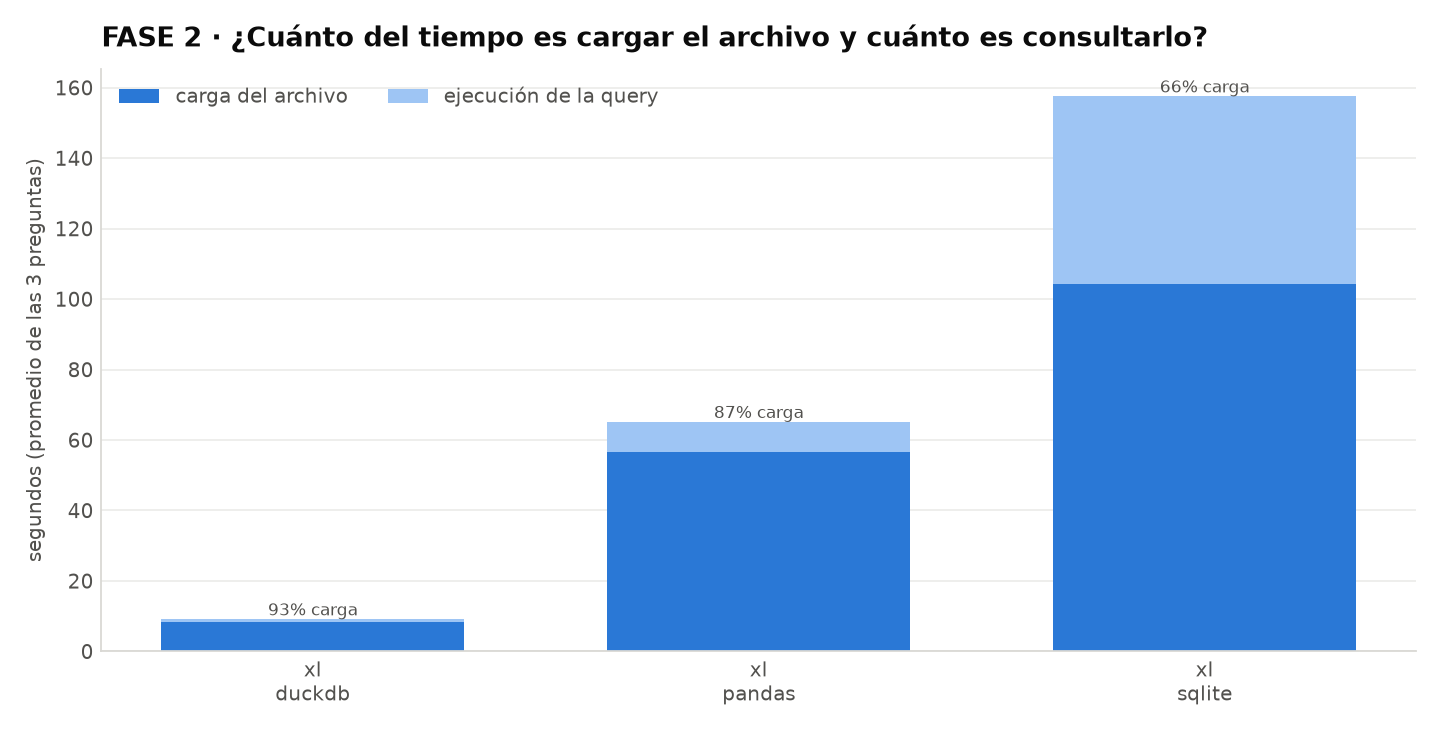
\includegraphics[width=0.75\textwidth]{figuras/fase2_carga_vs_query_pc_jesus.png}
  \caption{Reparto entre tiempo de carga y tiempo de consulta, Pc\_Jesus.}
  \label{fig:fase2-carga-query}
\end{figure}

\begin{figure}[htbp]
  \centering
  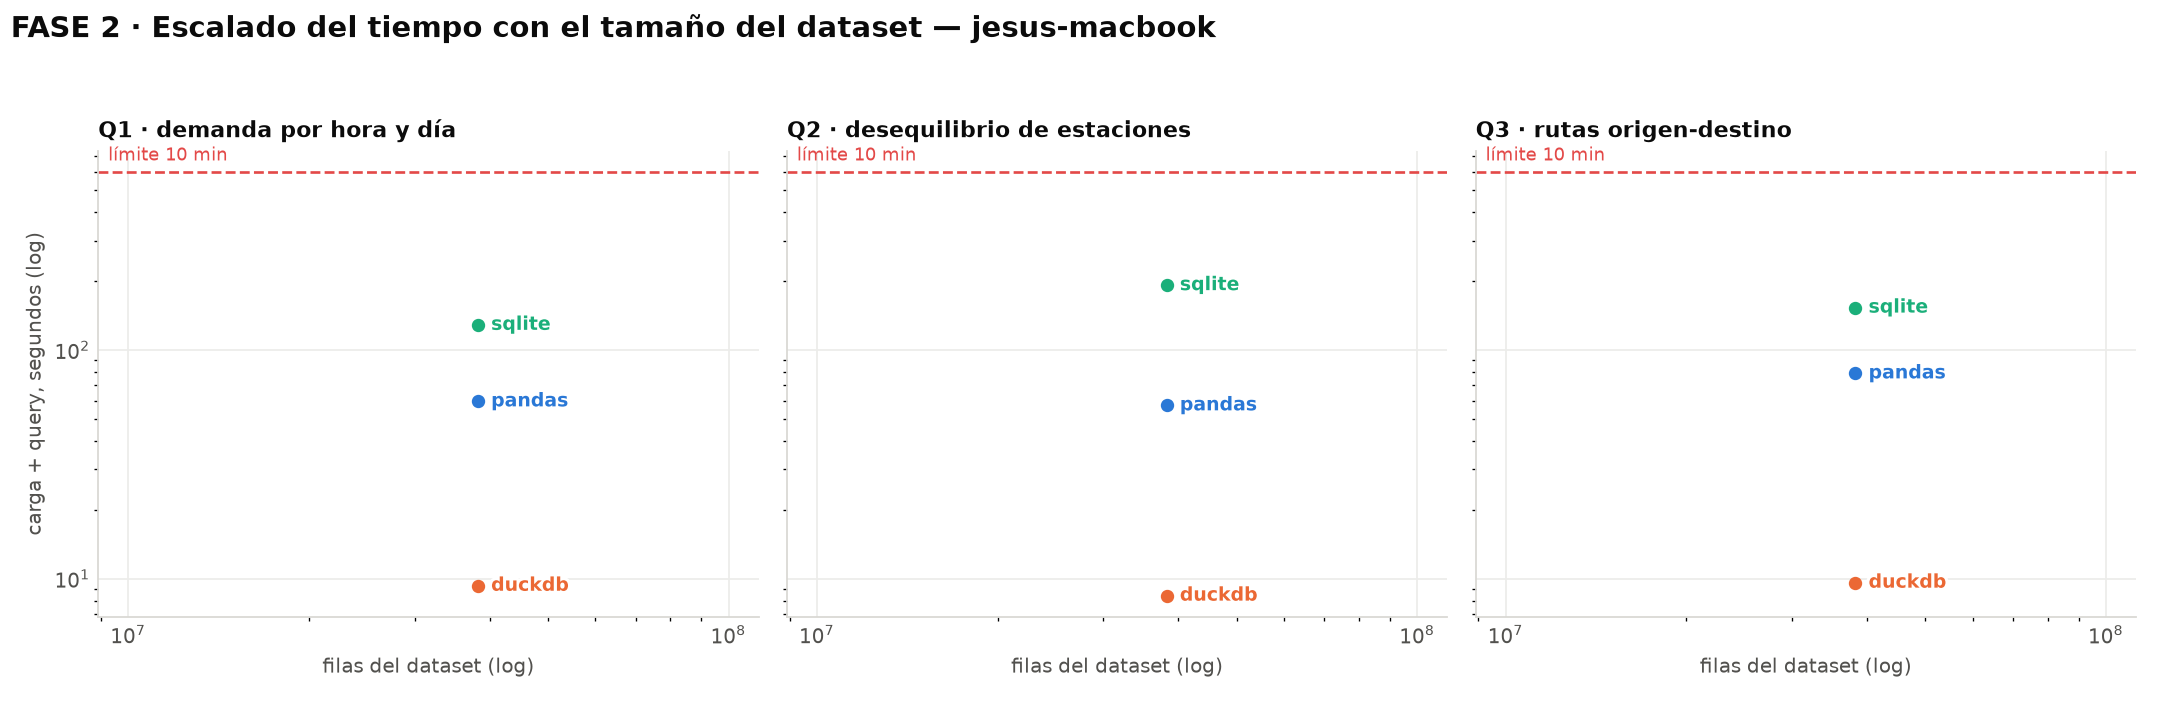
\includegraphics[width=0.75\textwidth]{figuras/fase2_escalado_pc_jesus.png}
  \caption{Escalado log-log del tiempo total contra el número de filas, Pc\_Jesus.}
  \label{fig:fase2-escalado}
\end{figure}

\section{Fase 3: Optimización}

Un paso de ETL ejecutado una sola vez por versión reduce el tiempo de análisis entre $10\times$ y $110\times$, y se amortiza antes de completar una sola corrida.

\subsection{Diagnóstico}

De la Fase 2 salen cuatro hechos que definen qué optimizar:

\begin{enumerate}
  \item La carga domina el tiempo total, y como cada pregunta recarga el archivo, ese costo se paga tres veces.
  \item Se leen nueve columnas y solo se usan tres: \texttt{start\_rental\_date\_time}, \texttt{start\_station\_id} y \texttt{end\_station\_id}. Las dos columnas de nombres de estación son las más pesadas y además son redundantes, porque ya están normalizadas en el catálogo.
  \item Los tipos están sobredimensionados. Los identificadores de estación llegan a $\sim$800 y viven en \texttt{INT64} o \texttt{DOUBLE}; la hora y el día se recalculan desde el timestamp en cada consulta.
  \item SQLite recorre filas completas y parsea timestamps con \texttt{strftime} registro por registro.
\end{enumerate}

\subsection{La optimización elegida}

Pre-procesar a un artefacto columnar con tipos reducidos, sobre el cual corren después todas las consultas.

\begin{table}[htbp]
\centering
\footnotesize
\caption{Decisiones de la optimización}
\label{tab:fase3-decisiones}
\begin{tabularx}{\textwidth}{>{\raggedright\arraybackslash}p{4.2cm}X}
\toprule
Decisión & Por qué mejora el rendimiento \\
\midrule
Formato Parquet, para Pandas y DuckDB & Binario y columnar: el motor lee solo las columnas de la consulta y no parsea texto. Trae esquema y tipos embebidos, así que no hay inferencia. \\
CSV estrecho de 4 enteros, para SQLite & SQLite no lee Parquet. Su artefacto es un CSV con cuatro columnas numéricas cortas: el parseo por fila se abarata frente a nueve campos con dos cadenas largas y dos timestamps. \\
Proyección a 4 columnas & Se eliminan \texttt{rental\_id}, \texttt{bike\_id}, \texttt{duration}, los dos nombres y \texttt{end\_rental\_date\_time}. Menos bytes leídos por fila. \\
Pre-cálculo de \texttt{dia\_semana} y \texttt{hora} & Se hace una vez en el ETL en vez de en cada consulta, y se guardan como \texttt{TINYINT}. \\
Tipos reducidos (\texttt{TINYINT}, \texttt{SMALLINT}) & Menos memoria por fila y mejor aprovechamiento de caché. \\
Ordenar por \texttt{dia\_semana, hora} & Potencia la codificación RLE de Parquet y reduce el tamaño en disco. \\
Índice covering por pregunta en SQLite & Cada consulta recibe únicamente el índice que necesita, en vez de construir tres y usar uno. \\
\bottomrule
\end{tabularx}
\end{table}

El artefacto Parquet de la versión XL pesa 89 MB frente a los 4,725 MB del CSV original: una reducción de $53\times$.

\subsection{Impacto medido}

Tiempo total de las tres preguntas, antes y después, en segundos.

\begin{table}[htbp]
\centering
\footnotesize
\caption{Impacto de la optimización por versión y equipo}
\label{tab:fase3-impacto}
\begin{tabularx}{\textwidth}{llXXXr}
\toprule
Versión & Equipo & Pandas & DuckDB & SQLite & ETL (s) \\
\midrule
M  & Pc\_Jesus  & $34.5$ a $0.7$ ($48\times$) & $5.0$ a $0.6$ ($8\times$) & $108.2$ a $61.7$ ($1.8\times$) & 8.4 \\
M  & Pc\_Martha & $50.0$ a $2.5$ ($20\times$) & $6.7$ a $2.0$ ($3\times$) & $164.6$ a $184.4$ ($0.9\times$) & 2.9 \\
M  & Pc\_Nahin  & $143.1$ a $3.9$ ($36\times$) & $15.3$ a $3.8$ ($4\times$) & $445.0$ a $221.7$ ($2.0\times$) & 8.4 \\
L  & Pc\_Jesus  & $79.1$ a $3.2$ ($25\times$) & $11.5$ a $1.0$ ($11\times$) & $232.8$ a $129.4$ ($1.8\times$) & 2.6 \\
L  & Pc\_Martha & $106.5$ a $4.6$ ($23\times$) & $15.3$ a $2.7$ ($6\times$) & $404.0$ a $304.1$ ($1.3\times$) & 5.4 \\
L  & Pc\_Nahin  & $288.1$ a $6.0$ ($48\times$) & $25.9$ a $6.5$ ($4\times$) & $776.9$ a $483.8$ ($1.6\times$) & 5.4 \\
XL & Pc\_Jesus  & $195.4$ a $3.4$ ($57\times$) & $27.3$ a $2.7$ ($10\times$) & $472.6$ a $291.5$ ($1.6\times$) & 6.3 \\
XL & Pc\_Martha & falló a $6.0$ & falló a $3.1$ & falló a $486.0$ & 10.6 \\
XL & Pc\_Nahin  & $501.4$ a $14.4$ ($35\times$) & $122.3$ a $14.6$ ($8\times$) & ver nota \S\ref{sec:nota-nahin} & 14.8 \\
\bottomrule
\end{tabularx}
\end{table}

En Pc\_Jesus, versión XL, las mejoras por pregunta llegan a $110\times$ en Pandas Q2 (57.1 s a 0.52 s).

\subsection{Amortización del ETL}

El ETL se paga una sola vez y el ahorro se cobra en cada corrida posterior. En la versión XL sobre Pc\_Jesus, el ETL cuesta 6.3 s y ahorra 191.9 s por corrida en Pandas: \textbf{se amortiza en el 3\% de una corrida}. En DuckDB, que ya era rápido, el ahorro es de 24.6 s por corrida y la amortización toma el 26\% de una corrida. En un pipeline que se ejecuta a diario la inversión se recupera de inmediato; para un análisis único aislado, el cálculo es menos evidente, y ese contraste es parte del resultado.

\subsection{Nota sobre SQLite en la versión XL de Pc\_Nahin}
\label{sec:nota-nahin}

Una lectura superficial de la gráfica sugiere que la optimización empeoró SQLite en esa máquina: 1,099.2 s en base contra 1,157.8 s optimizado. \textbf{La comparación no es válida.} En la etapa base, Q2 tardó 678.7 s y quedó marcada como \texttt{EXCEDE} por superar los 10 minutos, lo que hizo que el harness omitiera automáticamente Q3. Ese 1,099.2 es la suma de \textbf{dos} preguntas; el 1,157.8 es la suma de \textbf{tres}.

Comparando pregunta contra pregunta:

\begin{table}[htbp]
\centering
\caption{SQLite XL en Pc\_Nahin, comparación pregunta contra pregunta}
\label{tab:nahin-sqlite}
\begin{tabular}{lrrl}
\toprule
Pregunta & Base (s) & Optimizado (s) & Mejora \\
\midrule
Q1 & 420.5 & 237.8 & $1.77\times$ \\
Q2 & 678.7 (EXCEDE) & 539.5 & $1.26\times$ \\
Q3 & no ejecutada & 380.5 & de imposible a viable \\
\bottomrule
\end{tabular}
\end{table}

La optimización no solo ayudó: convirtió una ejecución que violaba el límite del enunciado en una que lo cumple.

\subsection{Por qué SQLite gana menos que las demás}

SQLite es la herramienta más castigada en la línea base y la que más gana en términos absolutos con el esquema estrecho. Pero \textbf{su ingesta sigue siendo proporcional al número de filas}: el \texttt{executemany} tiene que insertar los mismos millones de registros, solo que con campos más baratos de parsear. Por eso su mejora es grande pero no del orden de la de Pandas, y sigue sin alcanzar a DuckDB.

En Pc\_Martha, versión M, la optimización incluso resultó marginalmente más lenta (164.6 s contra 184.4 s). La causa es que construir el índice covering sobre 9.6 millones de filas cuesta más de lo que ahorra el parseo del CSV estrecho en esa máquina. \textbf{Una optimización no es universalmente buena: su valor depende de dónde estaba el cuello de botella.}

\begin{figure}[htbp]
  \centering
  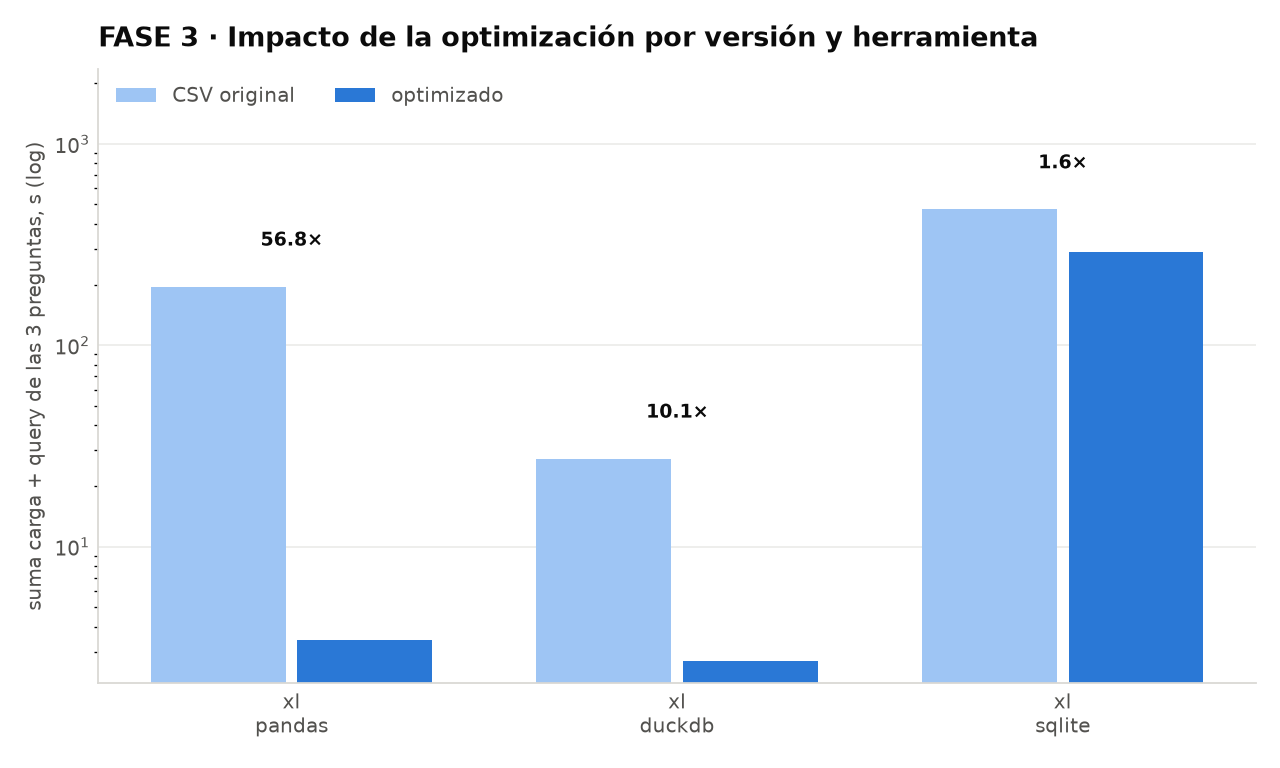
\includegraphics[width=0.75\textwidth]{figuras/fase3_impacto_pc_jesus.png}
  \caption{Impacto de la optimización por herramienta, Pc\_Jesus (base vs. optimizado).}
  \label{fig:fase3-impacto}
\end{figure}

\section{Comparación entre equipos}

Esta es la sección que responde la pregunta central del módulo: \textbf{¿en qué punto un problema se vuelve Big Data?} La respuesta que arrojan las mediciones es que no existe un punto, sino un umbral distinto por máquina y por representación de los datos.

\subsection{Dónde se rompe cada máquina}

\begin{table}[htbp]
\centering
\footnotesize
\caption{Punto de quiebre por equipo}
\label{tab:quiebre}
\begin{tabularx}{\textwidth}{lrXX}
\toprule
Equipo & RAM & Punto de quiebre en línea base & Con el artefacto optimizado \\
\midrule
Pc\_Jesus  & 8.0 GB & Ninguno. Completó M, L y XL en las tres herramientas & Completó todo \\
Pc\_Martha & 15.7 GB & \textbf{Falló en XL a los 17 minutos}, antes de terminar de leer el CSV & Completó XL en 6.0 s con Pandas \\
Pc\_Nahin  & 39.4 GB & SQLite cruzó los 10 minutos en XL Q2 (678.7 s) y arrastró la omisión de Q3 & Completó las tres preguntas \\
\bottomrule
\end{tabularx}
\end{table}

\subsection{Las tres lecturas}

\textbf{La máquina con menos RAM sobrevivió donde una con el doble falló.} El MacBook de 8 GB completó la versión XL en las tres herramientas, mientras el equipo de 15.7 GB abortó leyendo el mismo archivo. La memoria unificada y la velocidad del SSD compensaron la diferencia nominal de RAM. Esto descarta la lectura ingenua de que más memoria significa mayor capacidad de procesamiento.

\textbf{Cambiar la representación movió el umbral sin tocar el hardware.} La misma Pc\_Martha que no pudo leer el CSV de 4.7 GB procesó la versión XL en 6.0 segundos sobre el Parquet. El dataset no cambió, la máquina no cambió, solo cambió cómo estaban escritos los bytes. Si el umbral de Big Data se puede mover con un paso de ETL, entonces el umbral nunca fue una propiedad del dataset.

\textbf{La arquitectura del motor domina sobre las especificaciones del equipo.} DuckDB en la máquina de 8 GB (2.7 s en XL optimizado) superó ampliamente a SQLite en la máquina de 40 GB (varios minutos). Estructurar bien los datos y elegir un motor analítico adecuado rinde más que agregar memoria.

\subsection{Escalado}

En escala logarítmica, una recta de pendiente 1 indica escalado lineal $O(n)$. Lo relevante no es la pendiente sino dónde se rompe la linealidad: cuando los datos dejan de caber cómodamente en RAM, el sistema pagina a disco y la curva se dispara. Ese quiebre es distinto en cada máquina y es, precisamente, la frontera del Big Data para ese equipo.

\section{Respuestas a las tres preguntas}

Las tres herramientas producen resultados idénticos, ya validados celda a celda, así que las respuestas se calculan una sola vez sobre la \textbf{versión XL: 38,215,560 viajes}, la más grande disponible.

\subsection{Q1: Demanda por hora del día y día de la semana}

\textbf{El patrón es bimodal en días laborables y unimodal en fin de semana.} La forma de las dos curvas es distinta, y esa diferencia es la respuesta.

De lunes a viernes aparecen dos picos de desplazamiento al trabajo: \textbf{08:00 h} con un promedio de 710,450 viajes y \textbf{17:00-18:00 h} con 660,092 y 606,309. Sábado y domingo tienen un único máximo aplanado a las \textbf{14:00 h}, con 439,431 viajes promedio: uso recreativo, no de transporte.

\begin{table}[htbp]
\centering
\caption{Hora pico y total por día de la semana}
\label{tab:q1-picos}
\begin{tabular}{lrrr}
\toprule
Día & Hora pico & Viajes en la hora pico & Total del día \\
\midrule
Lunes     & 17:00 & 672,240 & 5,590,150 \\
Martes    & 08:00 & 768,730 & 5,902,367 \\
Miércoles & 08:00 & 741,295 & 5,795,257 \\
Jueves    & 08:00 & 742,080 & 5,795,656 \\
Viernes   & 08:00 & 645,178 & 5,633,146 \\
Sábado    & 14:00 & 442,283 & 4,914,592 \\
Domingo   & 14:00 & 436,579 & 4,584,392 \\
\bottomrule
\end{tabular}
\end{table}

El pico laborable es 1.62 veces el pico de fin de semana. El valle nocturno está a las 03:00 h con 8,638 viajes promedio, y la franja de 00:00 a 05:00 h concentra apenas el \textbf{2.0\% del uso semanal}.

\textbf{Uso operativo:} las horas pico marcan cuándo la flota debe estar completa. La franja nocturna, con un 2\% del tráfico, es la ventana natural para mantenimiento y rebalanceo sin afectar el servicio.

Una advertencia de interpretación: el rango de fechas depende de la versión. Las versiones chicas cubren pocas semanas y pueden caer en período navideño, donde el patrón laborable aparece atenuado porque varios días hábiles son feriados. Comparar el mapa de calor entre versiones es en sí mismo un resultado, porque muestra que con pocos datos se puede llegar a una conclusión equivocada sobre estacionalidad.

\begin{figure}[htbp]
  \centering
  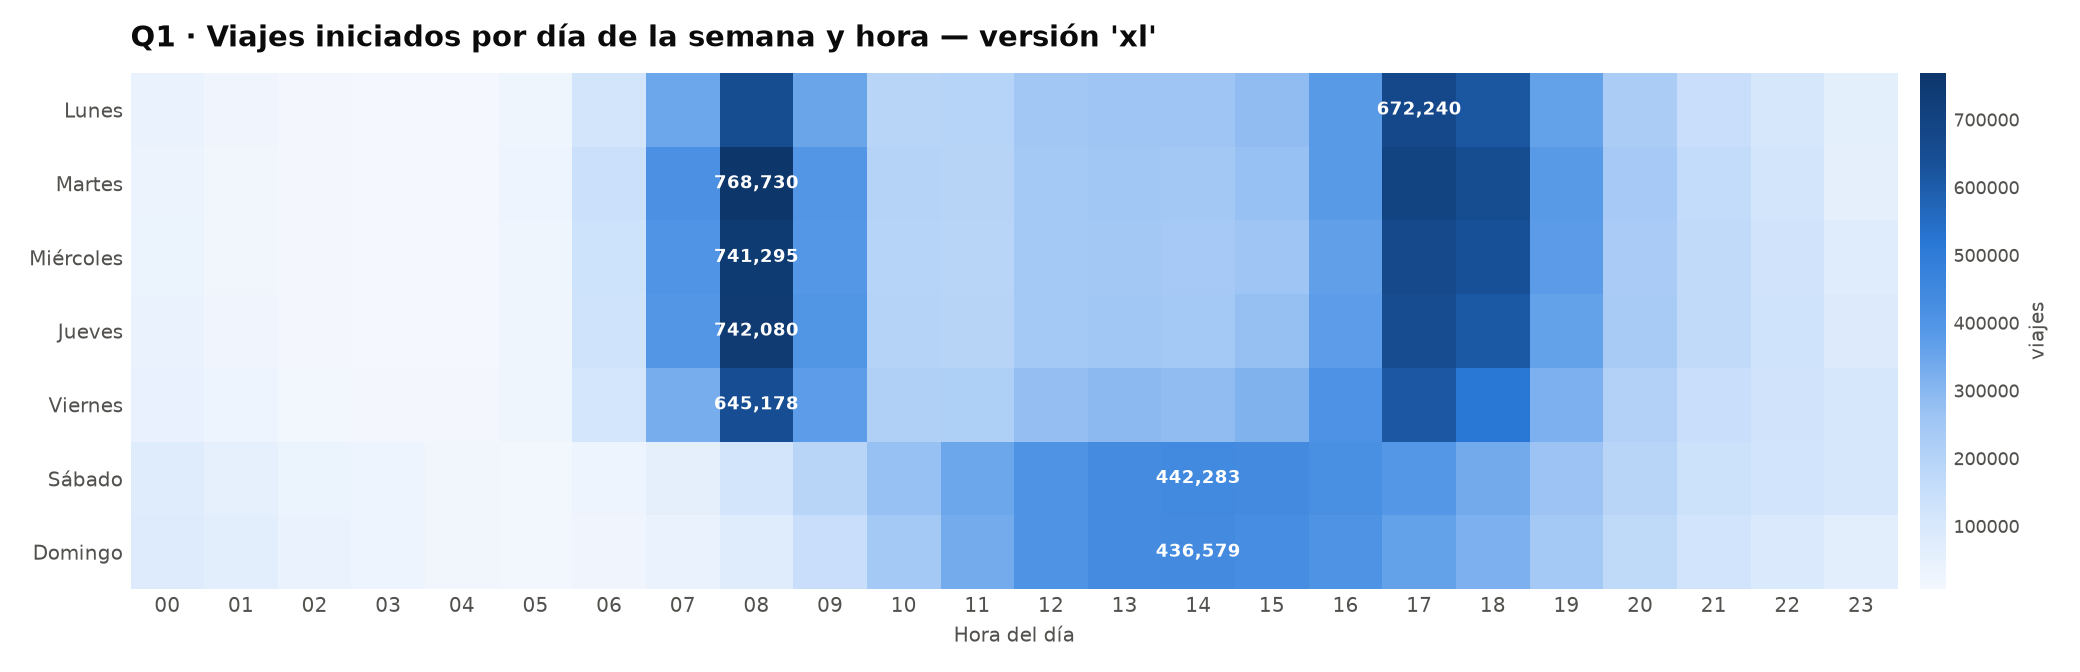
\includegraphics[width=0.8\textwidth]{figuras/q1_heatmap_xl.png}
  \caption{Mapa de calor de viajes por día de la semana y hora, versión XL.}
  \label{fig:q1-heatmap}
\end{figure}

\begin{figure}[htbp]
  \centering
  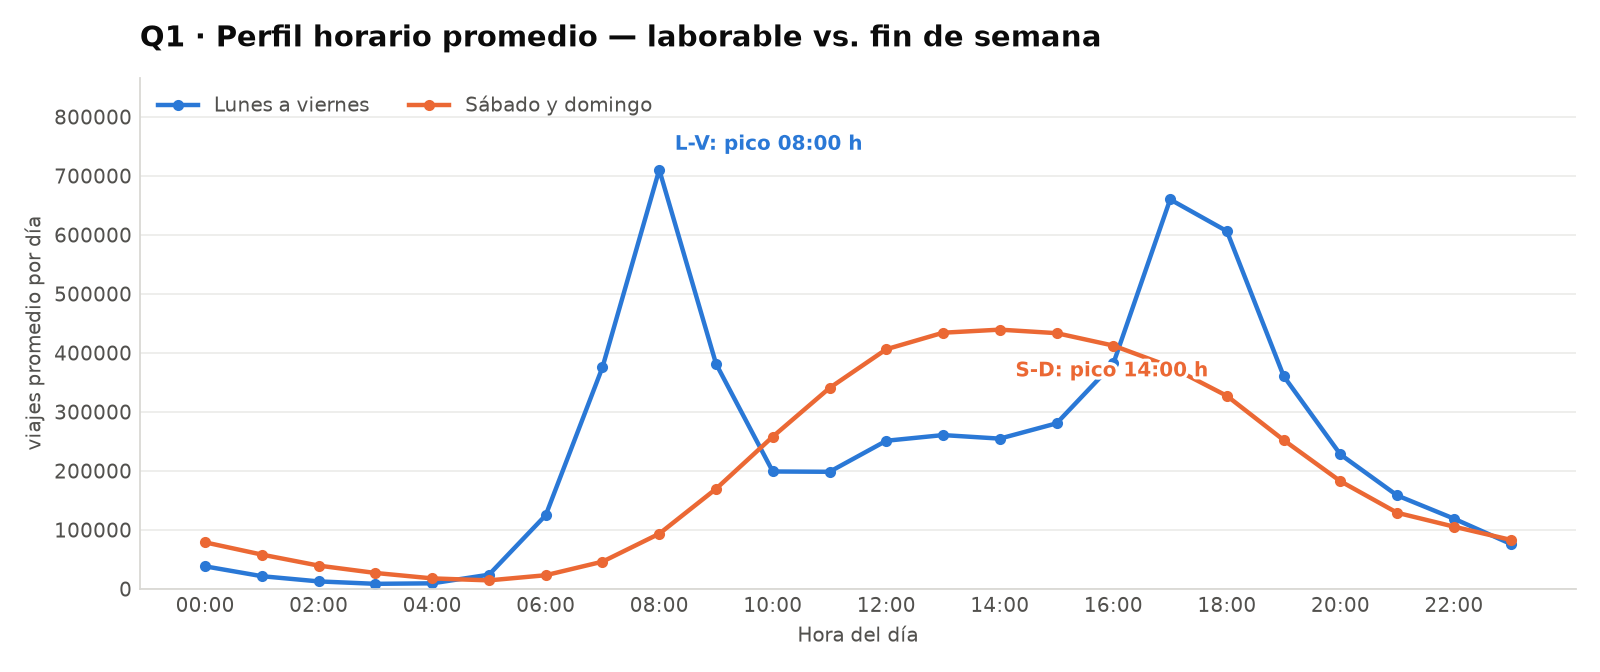
\includegraphics[width=0.8\textwidth]{figuras/q1_perfil_horario_xl.png}
  \caption{Perfil horario: días laborables vs. fin de semana, versión XL.}
  \label{fig:q1-perfil}
\end{figure}

\FloatBarrier

\subsection{Q2: Estaciones con mayor desequilibrio}

\textbf{El desbalance sigue el patrón radial clásico: déficit en nodos de transporte y periferia residencial, superávit en el núcleo financiero y comercial.} Con neto $=$ llegadas $-$ salidas, un valor negativo significa que la estación se vacía y hay que abastecerla; uno positivo, que se satura y hay que retirar bicicletas.

\begin{table}[htbp]
\centering
\footnotesize
\caption{Las cinco estaciones que más se vacían}
\label{tab:q2-deficit}
\begin{tabular}{lrrrr}
\toprule
Estación & Salidas & Llegadas & Neto & Desequilibrio \\
\midrule
Waterloo Station 2, Waterloo & 125,584 & 87,133 & $-38,451$ & $-18.1\%$ \\
Eagle Wharf Road, Hoxton & 107,628 & 86,866 & $-20,762$ & $-10.7\%$ \\
Cloudesley Road, Angel & 43,919 & 26,874 & $-17,045$ & $-24.1\%$ \\
Knightsbridge, Hyde Park & 51,202 & 37,693 & $-13,509$ & $-15.2\%$ \\
Notting Hill Gate Station, Notting Hill & 89,800 & 77,283 & $-12,517$ & $-7.5\%$ \\
\bottomrule
\end{tabular}
\end{table}

\begin{table}[htbp]
\centering
\footnotesize
\caption{Las cinco estaciones que más se saturan}
\label{tab:q2-superavit}
\begin{tabular}{lrrrr}
\toprule
Estación & Salidas & Llegadas & Neto & Desequilibrio \\
\midrule
Hop Exchange, The Borough & 176,231 & 237,045 & $+60,814$ & $+14.7\%$ \\
Holborn Circus, Holborn & 117,818 & 174,057 & $+56,239$ & $+19.3\%$ \\
St. James's Square, St. James's & 99,768 & 131,601 & $+31,833$ & $+13.8\%$ \\
Brushfield Street, Liverpool Street & 147,822 & 178,519 & $+30,697$ & $+9.4\%$ \\
Soho Square, Soho & 123,236 & 146,180 & $+22,944$ & $+8.5\%$ \\
\bottomrule
\end{tabular}
\end{table}

Waterloo Station encabeza el déficit, lo que confirma el patrón: la gente llega en tren y toma una bicicleta hacia el centro por la mañana. Holborn, Borough y St. James's son distritos de oficinas, y ahí es donde esas bicicletas terminan.

\textbf{Magnitud absoluta contra magnitud relativa.} El neto ordena por volumen, pero el porcentaje revela estaciones medianas con desbalance proporcional severo. Filtrando a estaciones con más de 20,000 viajes, los casos más críticos en términos relativos son \textbf{New North Road 1, Hoxton ($-26.9\%$)}, \textbf{Risinghill Street, Angel ($-25.2\%$)} y \textbf{Cloudesley Road, Angel ($-24.1\%$)}. El barrio de Angel aparece tres veces: es una zona residencial que se vacía sistemáticamente cada mañana. Para operaciones el porcentaje suele importar más que el absoluto, porque una estación que pierde una cuarta parte de su inventario está vacía buena parte del día.

\textbf{Sesgo declarado:} 68,213 viajes (0.18\% del total) no tienen estación de destino registrada. Cuentan como salida y no como llegada, así que empujan el neto hacia el déficit. El efecto es pequeño frente a las magnitudes reportadas, pero existe.

\begin{figure}[htbp]
  \centering
  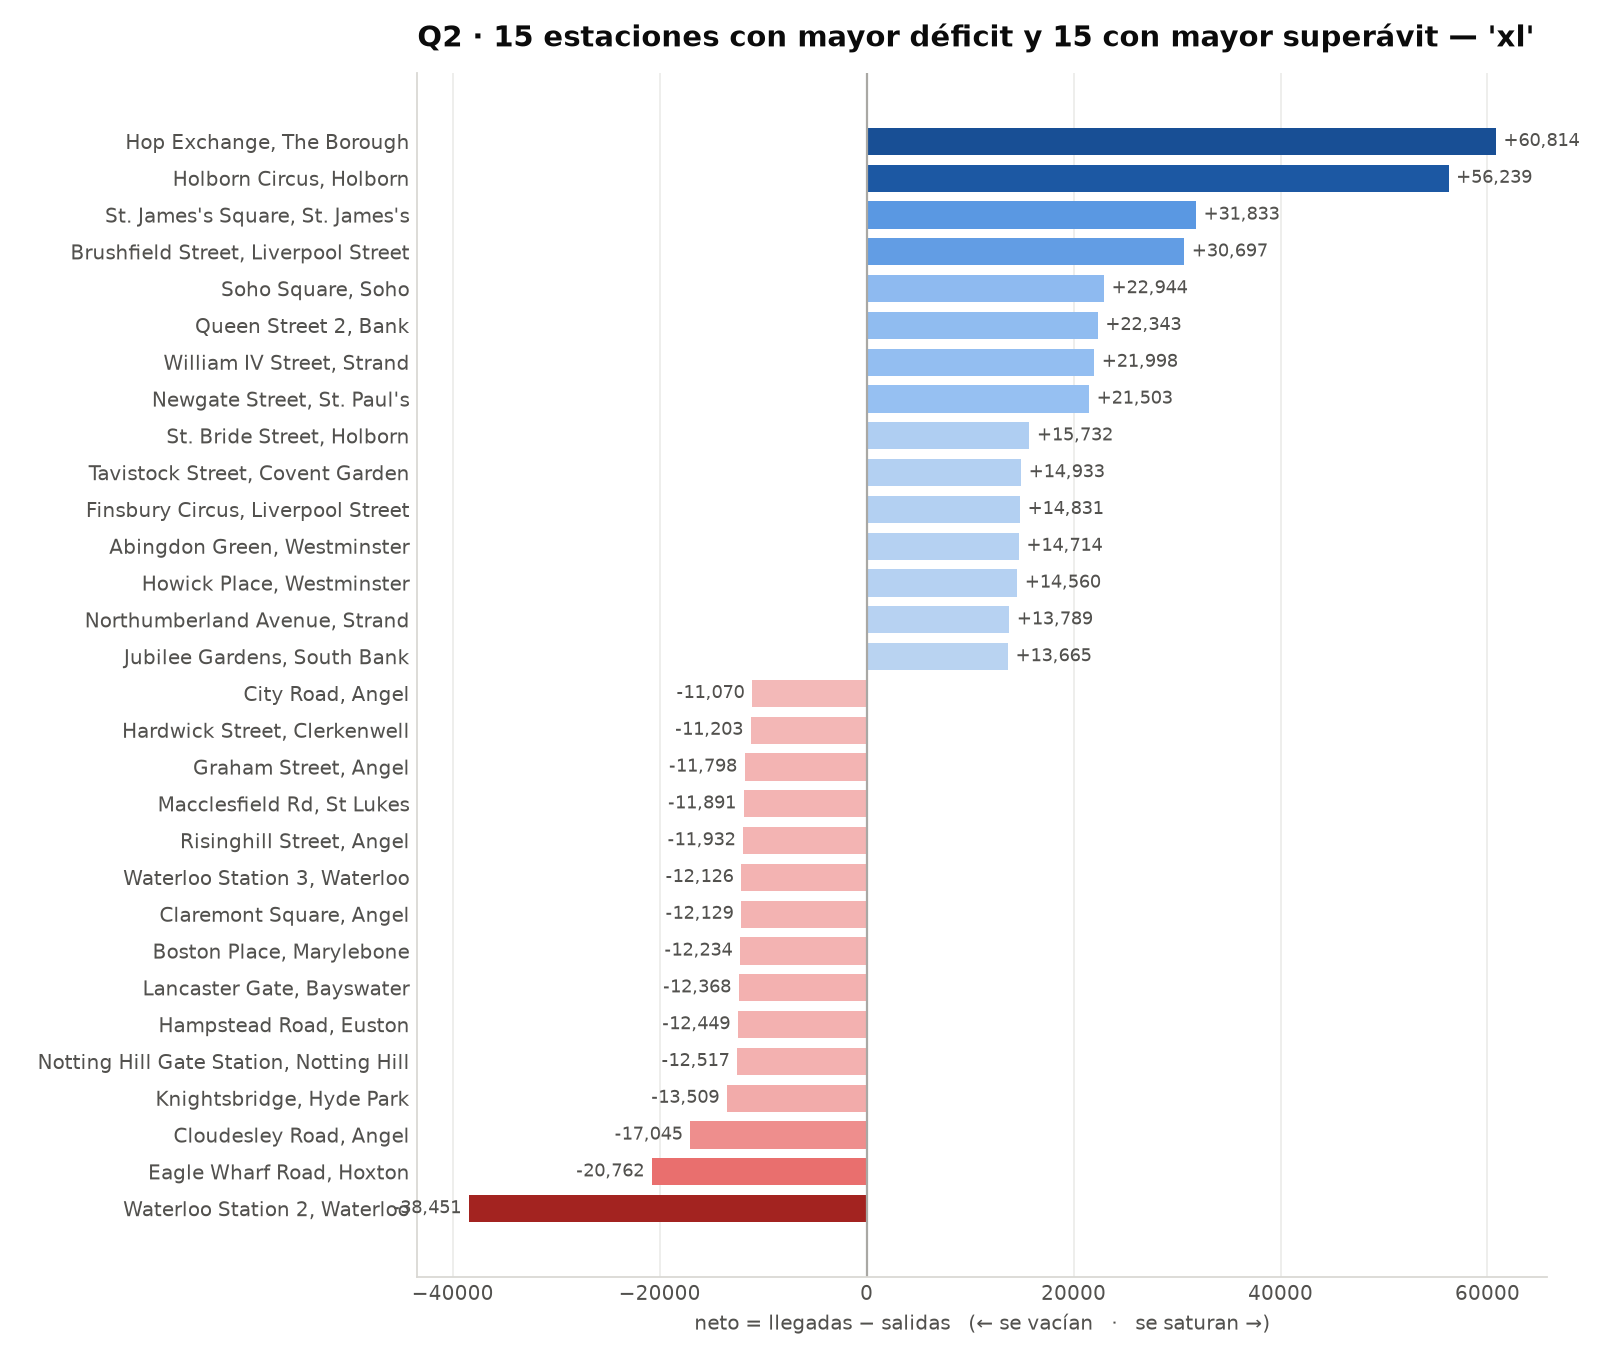
\includegraphics[width=0.8\textwidth]{figuras/q2_desequilibrio_xl.png}
  \caption{Estaciones con mayor déficit y superávit, versión XL.}
  \label{fig:q2-desequilibrio}
\end{figure}

\begin{figure}[htbp]
  \centering
  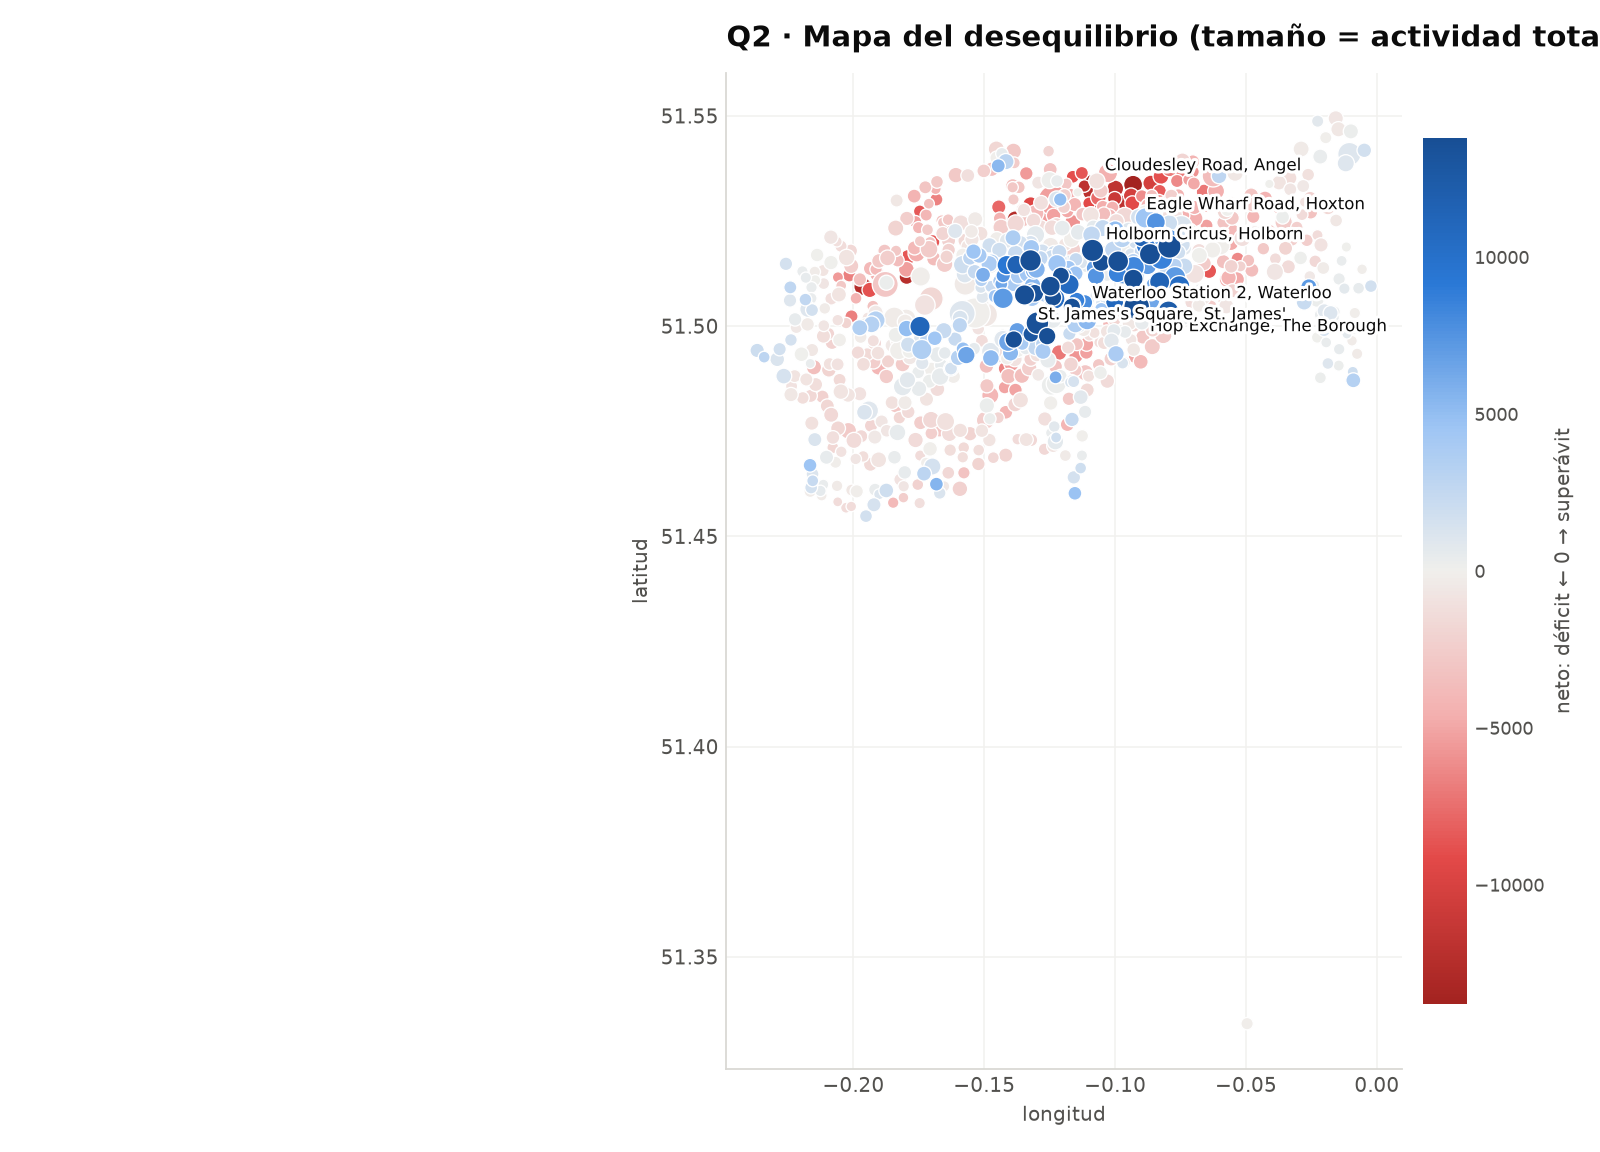
\includegraphics[width=0.8\textwidth]{figuras/q2_mapa_xl.png}
  \caption{Mapa geográfico del desbalance por estación, versión XL.}
  \label{fig:q2-mapa}
\end{figure}

\FloatBarrier

\subsection{Q3: Concentración del tráfico en rutas}

\textbf{Sí hay concentración, pero no es un Pareto 80/20: la forma es de cola extremadamente larga.} Sobre 652,864 pares origen-destino teóricamente posibles (808 estaciones al cuadrado), solo 510,672 aparecen alguna vez. Las \textbf{1,000 rutas más transitadas concentran el 9.6\% de todos los viajes}, y las 20 primeras apenas el 1.35\%.

\begin{table}[htbp]
\centering
\footnotesize
\caption{Rutas más transitadas, versión XL}
\label{tab:q3-rutas}
\begin{tabular}{clrr}
\toprule
\# & Ruta & Viajes & \% del total \\
\midrule
1  & Hyde Park Corner $\rightarrow$ Hyde Park Corner & 72,625 & 0.190\% \\
2  & Aquatic Centre $\rightarrow$ Aquatic Centre (Olympic Park) & 67,661 & 0.177\% \\
3  & Albert Gate $\rightarrow$ Albert Gate (Hyde Park) & 42,049 & 0.110\% \\
4  & Black Lion Gate $\rightarrow$ Black Lion Gate (Kensington Gardens) & 40,221 & 0.105\% \\
5  & Triangle Car Park $\rightarrow$ Triangle Car Park (Hyde Park) & 35,652 & 0.093\% \\
10 & Hyde Park Corner $\rightarrow$ Triangle Car Park & 15,739 & 0.041\% \\
11 & Hyde Park Corner $\rightarrow$ Albert Gate & 15,405 & 0.040\% \\
\bottomrule
\end{tabular}
\end{table}

Tres lecturas:

\begin{enumerate}
  \item \textbf{Las rutas circulares dominan el top y no son viajes de transporte.} Las nueve rutas más transitadas tienen origen igual a destino, y todas están en parques: Hyde Park, Kensington Gardens y el Queen Elizabeth Olympic Park. Son paseos recreativos, no desplazamientos. En las primeras 1,000 rutas hay 208 circulares que suman 1,026,226 viajes. Mezclarlas con los desplazamientos punto a punto distorsiona cualquier conclusión sobre movilidad, así que se marcan aparte.
  \item \textbf{Los corredores estructurales aparecen después.} Las rutas no circulares del top conectan puntos dentro de los mismos parques o nodos de transporte con distritos de oficinas. Son el último tramo del trayecto al trabajo y candidatas naturales a carril exclusivo o a más capacidad de anclajes.
  \item \textbf{La cola larga justifica la red.} Que ninguna ruta individual supere el 0.2\% del tráfico significa que el valor del sistema está en la cobertura, no en unos pocos corredores. Optimizar unas decenas de rutas tiene impacto local; mantener la red completa es lo que la hace útil como red.
\end{enumerate}

\textbf{Relación entre Q2 y Q3.} Una ruta asimétrica, con mucho tráfico A$\rightarrow$B y poco B$\rightarrow$A, es la \textbf{causa} del desequilibrio que Q2 mide como \textbf{efecto}. Cruzar ambas identifica qué corredor concreto genera cada estación deficitaria, que es la información que necesita el equipo de rebalanceo. Y cruzar Q2 con Q1 daría la ventana horaria en que conviene intervenir, porque una estación puede vaciarse por la mañana y llenarse por la tarde.

\begin{figure}[htbp]
  \centering
  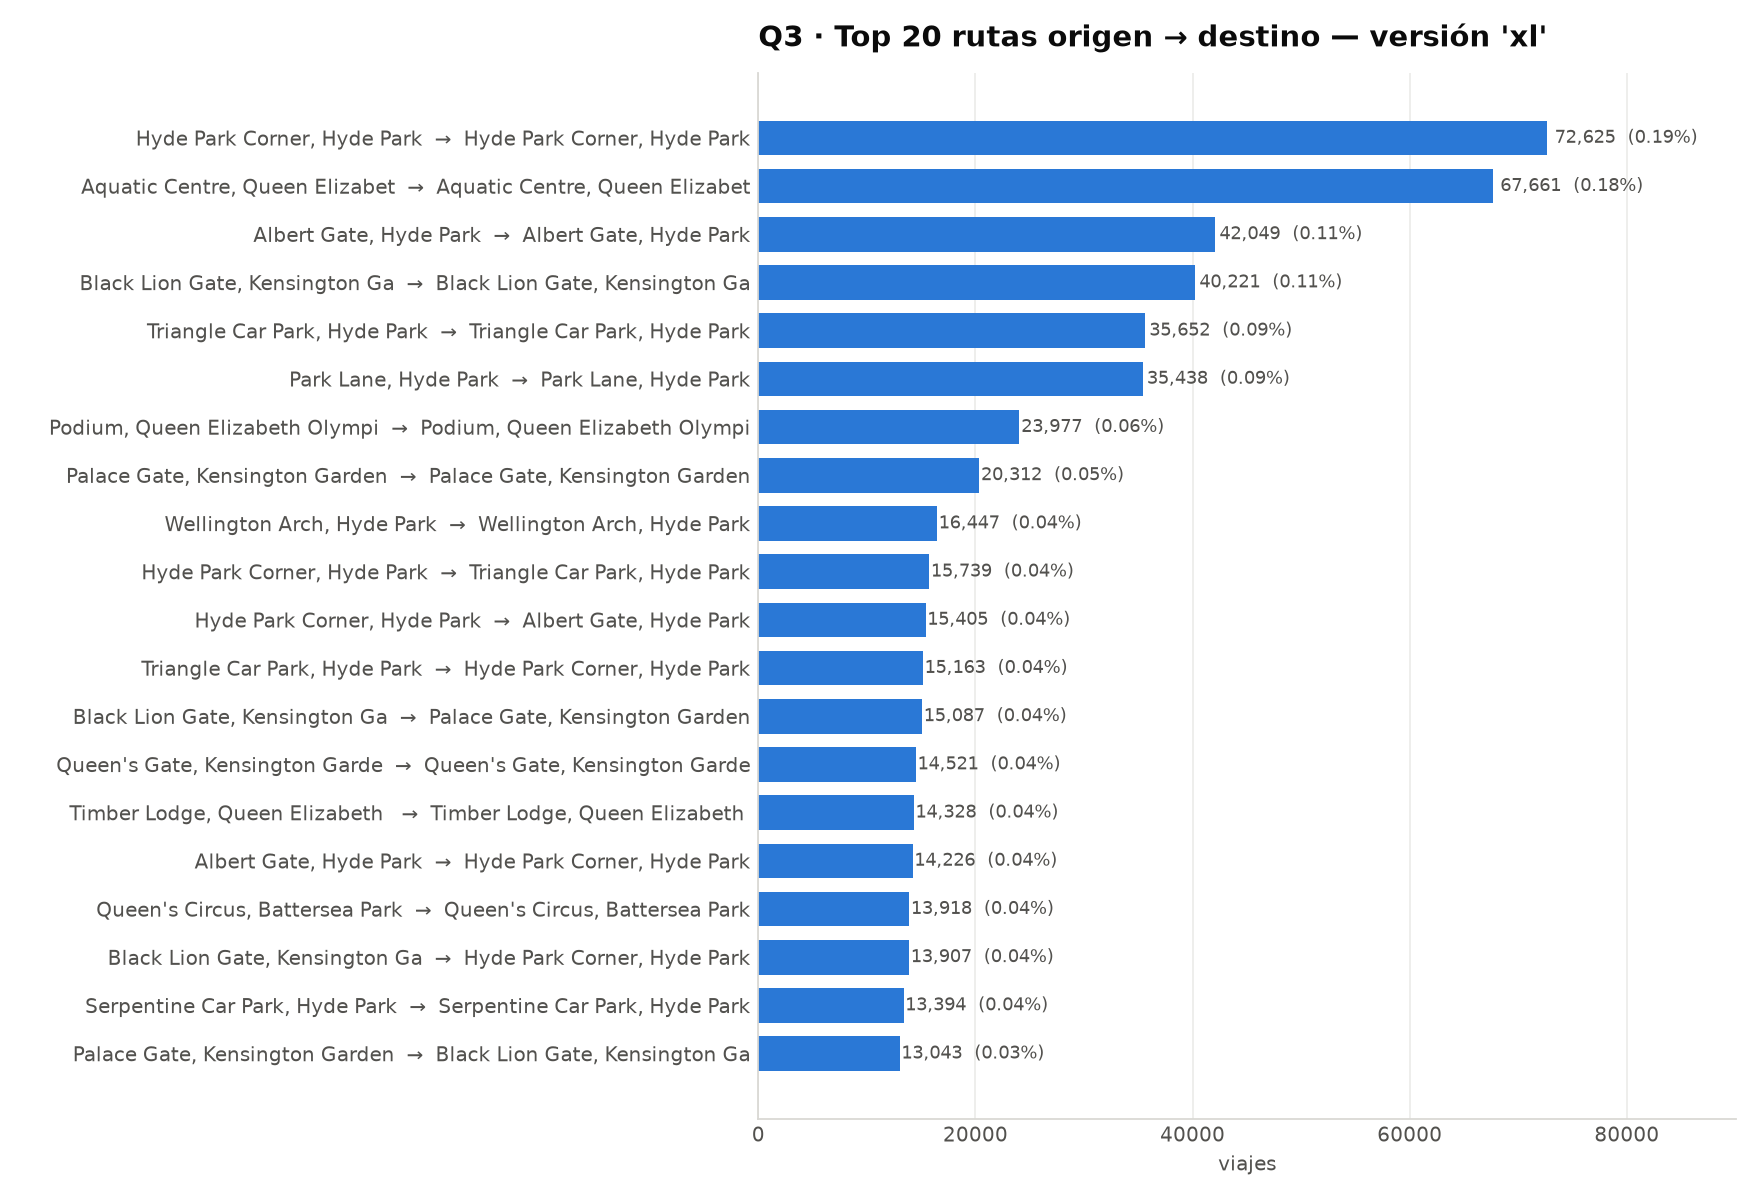
\includegraphics[width=0.8\textwidth]{figuras/q3_top_rutas_xl.png}
  \caption{Top 20 rutas más transitadas, versión XL.}
  \label{fig:q3-toprutas}
\end{figure}

\begin{figure}[htbp]
  \centering
  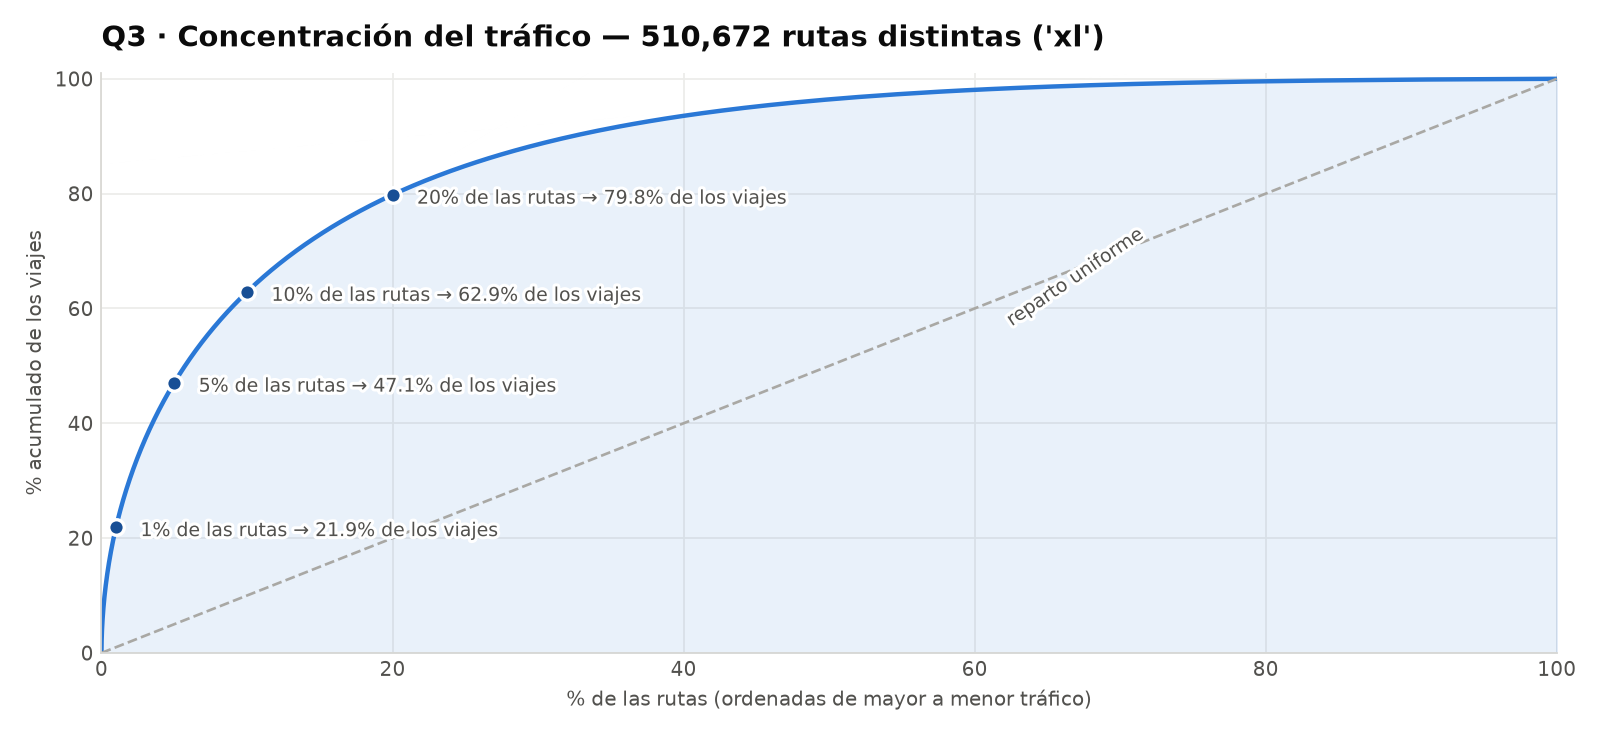
\includegraphics[width=0.8\textwidth]{figuras/q3_pareto_xl.png}
  \caption{Curva de concentración (Pareto) del tráfico por ruta, versión XL.}
  \label{fig:q3-pareto}
\end{figure}

\section{Diseño del pipeline ETL}
\label{sec:pipeline}

\begin{pendiente}
El enunciado pide únicamente el diagrama, sin implementación. Lo que sigue es una propuesta de partida basada en lo que ya se construyó en la Fase 3, con herramientas concretas de AWS asignadas a cada etapa; el equipo debe validarla y ajustarla.
\end{pendiente}

El ETL medido en la Fase 3 ya es, de hecho, un pipeline de una sola capa. Formalizarlo en capas lo vuelve reutilizable y explica las decisiones de diseño. Se asume un escenario de ingesta periódica: el operador del sistema de bicicletas entrega un archivo mensual con los viajes nuevos, de un tamaño similar a la versión S del dataset (0.488 GB, 3.97 millones de filas). Con esa cadencia, el archivo acumulado en la capa bronce alcanza el tamaño de la versión XL (4.725 GB) alrededor del mes 10, momento que se usa como estado estable para el análisis de costos de la Sección \ref{sec:costos}.

\begin{figure}[htbp]
\centering
\resizebox{\textwidth}{!}{%
\begin{tikzpicture}[
  node distance=1.0cm and 1.0cm,
  box/.style={draw, rounded corners, align=center, minimum height=2.4cm, minimum width=2.5cm, fill=blue!4, font=\footnotesize, text width=2.3cm},
  arr/.style={-{Stealth[length=2.2mm]}, thick}
]
  \node[box] (A) {\\[14pt] CSV mensual\\ \texttt{london.csv}\\ (fuente externa)};

  \node[box, right=of A] (B)
    {
\includegraphics[width=0.9cm]{figuras/aws-icons/eventbridge.pdf}\\[2pt]
     Ingesta\\ EventBridge\\ Scheduler};

  \node[box, right=of B] (C)
    {
\includegraphics[width=0.9cm]{figuras/aws-icons/s3.pdf}\\[2pt]
     Bronce\\ S3 \texttt{raw/}\\ 9 columnas};

  \node[box, right=of C] (D)
    {
\includegraphics[width=0.9cm]{figuras/aws-icons/glue.pdf}\\[2pt]
     Limpieza\\ AWS Glue\\ cast, nulos};

  \node[box, right=of D] (E)
    {
\includegraphics[width=0.9cm]{figuras/aws-icons/s3.pdf}\\[2pt]
     Plata\\ S3 \texttt{silver/}\\ Parquet};

  \node[box, right=of E] (F)
    {
\includegraphics[width=0.9cm]{figuras/aws-icons/glue.pdf}\\[2pt]
     Agregación\\ AWS Glue\\ \texttt{GROUP BY}};

  \node[box, right=of F] (G)
    {
\includegraphics[width=0.9cm]{figuras/aws-icons/s3.pdf}\\[2pt]
     Oro\\ S3 \texttt{gold/}\\ Q1 Q2 Q3};

  \node[box, above=of D, fill=green!5] (H)
    {
\includegraphics[width=0.9cm]{figuras/aws-icons/s3.pdf}\\[2pt]
     Catálogo\\ estaciones\\ S3, 802 filas};

  \node[box, right=of G, fill=orange!5] (I)
    {
\includegraphics[width=0.9cm]{figuras/aws-icons/athena.pdf}\\[2pt]
     Consumo\\ Athena +\\ QuickSight};

  \draw[arr] (A) -- (B);
  \draw[arr] (B) -- (C);
  \draw[arr] (C) -- (D);
  \draw[arr] (D) -- (E);
  \draw[arr] (E) -- (F);
  \draw[arr] (F) -- (G);
  \draw[arr] (H) -- (D);
  \draw[arr] (G) -- (I);
\end{tikzpicture}%
}
\caption{Pipeline ETL propuesto sobre AWS, capas medallón (bronce/plata/oro), con íconos oficiales de los servicios (Amazon S3, AWS Glue, Amazon EventBridge Scheduler, Amazon Athena) y entrada lateral del catálogo de estaciones en la etapa de limpieza.}
\label{fig:pipeline}
\end{figure}

\subsection{Herramientas y servicios por etapa}

\begin{table}[htbp]
\centering
\footnotesize
\caption{Servicios de AWS asignados a cada etapa del pipeline}
\label{tab:pipeline-herramientas}
\begin{tabularx}{\textwidth}{>{\raggedright\arraybackslash}p{2.1cm}>{\raggedright\arraybackslash}p{3.4cm}X}
\toprule
Etapa & Servicio & Por qué esa herramienta \\
\midrule
Orquestación & EventBridge Scheduler + Step Functions & Dispara el job mensual y coordina las etapas. Un entorno persistente de Airflow administrado (Amazon MWAA) cuesta más de \$300/mes solo por estar encendido, muy por encima del costo del job que orquesta; estos dos servicios cobran por invocación y caen en la capa gratuita a este volumen. \\
Ingesta / Bronce & S3 (bucket \texttt{raw/}) & Almacenamiento de objetos barato y duradero para el CSV tal cual llega, sin transformar. También aloja el catálogo de estaciones. \\
Limpieza y transformación & Glue (job PySpark) & Motor Spark serverless: resuelve el casteo de tipos, los nulos y la proyección a 4 columnas sin administrar un clúster; el mismo trabajo que Fase 3 hizo localmente, escalado a un servicio gestionado. \\
Plata & S3 (bucket \texttt{silver/}), Parquet & Sigue la decisión de Fase 3: Parquet columnar con tipos reducidos, que ya demostró $53\times$ de reducción frente al CSV. \\
Catálogo de esquema & Glue Data Catalog & Registra el esquema de plata para que Athena y Glue la lean sin definir tablas a mano. \\
Agregación / Oro & Glue (mismo job) & Calcula las tablas Q1, Q2 y Q3 y las escribe como Parquet pequeño en \texttt{gold/}. \\
Consumo & Athena (SQL) + QuickSight & Athena consulta directo sobre S3 sin mover datos ni levantar infraestructura; se paga solo por lo escaneado, mínimo en la capa oro. \\
\bottomrule
\end{tabularx}
\end{table}

La capa de limpieza es donde se resuelven los tres problemas de calidad detectados en la exploración: el casteo de \texttt{end\_station\_id} a entero, el tratamiento de los nulos de destino y el marcado de duraciones anómalas. La capa plata materializa la proyección de cuatro columnas con tipos reducidos que produjo las mejoras de la Fase 3.

\textbf{Pendiente de decidir por el equipo:}

\begin{itemize}
  \item Confirmar si el enunciado pide capas medallón u otra nomenclatura
  \item Decidir si el catálogo de estaciones se une en plata o en oro
  \item Especificar la estrategia de particionado en S3, si aplica (por ejemplo, por año-mes de \texttt{start\_rental\_date\_time})
\end{itemize}

\section{Análisis de costos}
\label{sec:costos}

El análisis cubre dos cosas distintas: el costo de operar el pipeline ETL propuesto en la Sección \ref{sec:pipeline} sobre AWS, y el costo ya medido de la optimización de la Fase 3. Los precios son los públicos de AWS para la región \texttt{us-east-1} (N. Virginia), consultados en septiembre de 2026; no se espera exactitud, sino que el desglose sea razonable y esté sustentado.

\textbf{Supuestos del escenario:}

\begin{itemize}
  \item Proveedor: AWS, región us-east-1. Precios bajo demanda (\emph{on-demand}), sin descuentos por compromiso.
  \item Frecuencia: batch mensual. Cada corrida ingiere un archivo del tamaño de la versión S (0.488 GB, 3.97 millones de filas), que es el ritmo de crecimiento asumido para el dataset real.
  \item Estado estable: mes 10, cuando el acumulado en la capa bronce alcanza el tamaño de la versión XL (4.725 GB), la más grande medida en este trabajo.
  \item La capa plata mantiene la razón de reducción de la Fase 3 ($53\times$ frente al CSV), así que el Parquet acumulado en el mes 10 pesa $\sim$89 MB.
\end{itemize}

\subsection{Costo del pipeline en la nube (mensual, estado estable)}

\begin{table}[htbp]
\centering
\footnotesize
\caption{Desglose de costo mensual del pipeline en AWS, mes 10 (estado estable)}
\label{tab:costos-nube}
\begin{tabularx}{\textwidth}{>{\raggedright\arraybackslash}p{3.1cm}Xrc}
\toprule
Componente & Cálculo & Costo/mes & Fuente \\
\midrule
Almacenamiento S3 (bronce+plata+oro) & $(4.725 + 0.089 + 0.005)$ GB $\times \$0.023$/GB & \$0.111 & \href{https://aws.amazon.com/s3/pricing/}{[1]} \\
Solicitudes S3 (PUT/GET mensuales) & $\sim$50 PUT $\times \$0.005/1000$ + $\sim$5{,}000 GET $\times \$0.0004/1000$ & \$0.002 & \href{https://aws.amazon.com/s3/pricing/}{[1]} \\
Cómputo ETL (AWS Glue, 1 corrida/mes) & 2 DPU $\times$ 10 min $\times \$0.44$/DPU-hora & \$0.147 & \href{https://aws.amazon.com/glue/pricing/}{[2]} \\
Orquestación (EventBridge + Step Functions) & Dentro de la capa gratuita a este volumen & \$0.000 & \href{https://aws.amazon.com/eventbridge/pricing/}{[3]} \\
Catálogo de esquema (Glue Data Catalog) & Dentro del millón de objetos gratuitos & \$0.000 & \href{https://aws.amazon.com/glue/pricing/}{[2]} \\
Consulta (Amazon Athena) & $\sim$2 GB escaneados/mes $\times \$5$/TB & \$0.010 & \href{https://aws.amazon.com/athena/pricing/}{[4]} \\
Transferencia de salida & Muy por debajo de los 100 GB/mes gratuitos & \$0.000 & \href{https://aws.amazon.com/ec2/pricing/on-demand/}{[5]} \\
\midrule
\textbf{Total estimado} & & \textbf{\$0.27/mes} & \\
\bottomrule
\end{tabularx}
\vspace{0.3em}
{\footnotesize [1] \url{aws.amazon.com/s3/pricing} \quad [2] \url{aws.amazon.com/glue/pricing} \quad [3] \url{aws.amazon.com/eventbridge/pricing} \quad [4] \url{aws.amazon.com/athena/pricing} \quad [5] \url{aws.amazon.com/ec2/pricing/on-demand}}
\end{table}

El total es minúsculo (menos de \$4 al año) porque todo el histórico del dataset cabe en menos de 5 GB. Esa es en sí misma una conclusión relevante: \textbf{a esta escala, el costo de nube no es un problema}; lo que domina el presupuesto es la decisión de diseño (Parquet vs. CSV, Glue serverless vs. un clúster fijo), no el gasto en infraestructura. Esto es consistente con el hallazgo de la Fase 3: la representación de los datos importa más que la cantidad de recursos que se les asigna.

\textbf{Sensibilidad a la escala.} Si el sistema creciera 200 veces (varias ciudades, varios años, $\sim$1 TB acumulado), el almacenamiento en bronce pasaría a $1{,}024\text{ GB} \times \$0.023 \approx \$23.6$/mes y el job de Glue pasaría de 10 minutos a un orden de magnitud más por corrida. El costo dejaría de ser trivial, pero seguiría siendo pequeño frente al costo de mantener SQLite sin optimizar corriendo minutos por consulta, como se documentó en la Fase 3.

\subsection{Costo ya medido: cómputo local y tiempo de persona}

\textbf{Costo en almacenamiento (medido).} El CSV original de la versión XL pesa 4,725 MB. El Parquet optimizado pesa 89 MB y el CSV estrecho para SQLite pesa 442 MB. La reducción es de $53\times$ y $10.7\times$ respectivamente.

\textbf{Costo en cómputo local (medido).} El ETL de la Fase 3 cuesta entre 2.6 s y 14.8 s según la máquina y la versión. El ahorro por corrida completa del análisis va de 24.6 s (DuckDB, XL) a 191.9 s (Pandas, XL). La amortización ocurre en una fracción de la primera corrida.

\textbf{Costo en tiempo de persona.} Pc\_Martha perdió 17 minutos en una ejecución que terminó fallando. Ese tipo de costo no aparece en ninguna tabla de benchmark ni en la tabla de costos de nube, pero es real y recurrente cada vez que alguien reproduce el análisis sin el artefacto optimizado.

\textbf{Pendiente de decidir por el equipo:}

\begin{itemize}
  \item Validar los supuestos de frecuencia y tamaño de la carga incremental contra el enunciado, si este especifica algo distinto
  \item Decidir si conviene reservar capacidad de Athena o Glue Flex si el volumen de consultas crece
\end{itemize}

\section{Problemas encontrados}

\begin{longtable}{>{\raggedright\arraybackslash}p{0.4cm}>{\raggedright\arraybackslash}p{7.9cm}>{\raggedright\arraybackslash}p{7.9cm}}
\caption{Problemas encontrados durante el desarrollo}
\label{tab:problemas} \\
\toprule
\# & Problema & Cómo se resolvió \\
\midrule
\endfirsthead
\multicolumn{3}{l}{\footnotesize \textit{Cuadro \thetable\ (continuación): Problemas encontrados durante el desarrollo}} \\
\toprule
\# & Problema & Cómo se resolvió \\
\midrule
\endhead
\bottomrule
\endfoot
\bottomrule
\endlastfoot
1 & \textbf{Las tres herramientas numeran los días de la semana distinto.} Pandas \texttt{dt.dayofweek} arranca en lunes $=0$; DuckDB \texttt{dayofweek()} y SQLite \texttt{strftime('\%w')} arrancan en domingo $=0$. Los resultados no coincidían aunque el total sí. &
Se unificó todo a lunes $=0$ con \texttt{isodow()-1} en DuckDB y \texttt{(strftime('\%w')+6)\%7} en SQLite. La validación cruzada se agregó justamente para cazar este tipo de error. \\
2 & \textbf{\texttt{end\_station\_id} se infiere como \texttt{DOUBLE}} porque tiene nulos, mientras \texttt{start\_station\_id} es entero. Al agrupar por el par, los identificadores no cruzaban: \texttt{529.0} contra \texttt{529}. &
\texttt{CAST(... AS BIGINT)} y \texttt{.astype(\textquotedbl int64\textquotedbl)} explícitos en las tres herramientas antes de agrupar. \\
3 & \textbf{\texttt{FULL OUTER JOIN} no existe en SQLite anterior a la versión 3.39.} La consulta de Q2, escrita originalmente para DuckDB, fallaba con error de sintaxis en instalaciones de SQLite más antiguas durante el desarrollo. &
Se reescribió con un CTE \texttt{ids} (unión de los identificadores de origen y destino) más dos \texttt{LEFT JOIN}, y se usó la misma forma en DuckDB para que las consultas fueran estructuralmente comparables. \\
4 & \textbf{La ingesta a SQLite era lentísima} con el journal y el \texttt{fsync} por defecto. &
\texttt{PRAGMA journal\_mode=OFF}, \texttt{synchronous=OFF}, \texttt{cache\_size=-262144} e inserción por lotes de 200,000 filas con \texttt{executemany}, en vez de un \texttt{INSERT} por fila. \\
5 & \textbf{SQLite no conserva el CSV cargado entre consultas}, a diferencia de Pandas y DuckDB. &
Se adoptó el protocolo de ejecución independiente y se aplicó a las tres herramientas, para que la comparación fuera simétrica. \\
6 & \textbf{El import de \texttt{pyarrow} inflaba el tiempo de carga del Parquet.} Pandas lo carga de forma perezosa en el primer \texttt{read\_parquet()}, y ese import en frío se contabilizaba como tiempo de lectura de datos. &
Se movió el import fuera de todo bloque cronometrado. \\
7 & \textbf{Los artefactos pesados en carpetas sincronizadas distorsionaban los tiempos.} La sincronización en segundo plano compite por I/O. &
Los \texttt{.db} y \texttt{.parquet} se escriben en disco local, no en la carpeta de nube. \\
8 & \textbf{Pc\_Martha (15.7 GB) falló en XL tras 17 minutos} sin llegar a completar la lectura del CSV. &
Se registró como resultado, no como error a corregir: es el dato que define el umbral de Big Data para ese equipo. Se corrió una segunda pasada sin XL para obtener la serie completa de las demás versiones. \\
9 & \textbf{La gráfica de impacto suma tiempos sin verificar que ambas etapas tengan las mismas preguntas completadas.} Cuando una etapa tiene ejecuciones omitidas, la barra de la línea base queda artificialmente corta y sugiere que la optimización empeoró el rendimiento. &
Se detectó en el caso de SQLite en XL sobre Pc\_Nahin y se corrigió comparando pregunta contra pregunta. La comparación válida está en la Fase 3 (\S\ref{sec:nota-nahin}). \\
\end{longtable}

\section{Limitaciones metodológicas}

Hay tres advertencias que condicionan cómo deben leerse los números de este informe.

La primera es que el pico de RAM no resulta comparable entre macOS y Windows. Pandas en XL reporta 4,522 MB en Pc\_Jesus y 12,096 MB en Pc\_Nahin para el mismo código y los mismos datos. macOS comprime páginas de memoria y el RSS que reporta \texttt{psutil} no las contabiliza, así que estas cifras sirven para comparar herramientas \textbf{dentro} de una misma máquina, pero no entre sistemas operativos.

La segunda es que el equipo de mayores especificaciones resultó el más lento. Pc\_Nahin (Core Ultra 9, 40 GB) tarda de 2 a 4 veces más que Pc\_Jesus (8 GB) en todas las herramientas, incluida la carga pura de CSV con DuckDB, que pasa de 8 a 36 segundos en XL. La brecha es de entrada/salida y no de CPU ni de memoria. Las causas plausibles son una carpeta sincronizada con la nube, un antivirus escaneando 4.7 GB en cada lectura, o las tres versiones corridas en una sola sesión sin liberar memoria. No se verificó cuál aplica, así que los tiempos absolutos de ese equipo deben tomarse como cota superior.

La tercera es que las versiones de librerías difieren entre equipos (Cuadro \ref{tab:software}). Eso no explica diferencias de orden de magnitud, pero sí introduce ruido en las comparaciones finas. Por eso las conclusiones de este informe se apoyan en órdenes de magnitud y en fallos categóricos, y no en márgenes estrechos.

\section{Conclusiones}

\textbf{Big Data no es un tamaño, es una relación.} El mismo archivo de 38.2 millones de filas fue imposible en una máquina de 15.7 GB de RAM y manejable en una de 8 GB. Ninguna cifra absoluta de filas o gigabytes marca la frontera; la marca la interacción entre el volumen, la forma en que están escritos los datos y el equipo que los procesa.

\textbf{La representación es la palanca más barata.} El paso de CSV a Parquet con proyección y tipos reducidos costó entre 2.6 y 14.8 segundos por versión y multiplicó el rendimiento por factores de hasta $110\times$. Más importante: movió el umbral de viabilidad. Un equipo que no podía procesar la versión completa pasó a hacerlo en 6 segundos, sin agregar hardware.

\textbf{La arquitectura del motor importa más que sus especificaciones.} DuckDB, columnar y vectorizado, resolvió en 2.7 segundos sobre 8 GB de RAM lo que SQLite, orientado a filas, no terminaba en 10 minutos sobre 40 GB. Los índices y los \texttt{PRAGMA} mejoran a SQLite, pero no cambian su modelo de almacenamiento: un B-tree no convierte un motor OLTP en columnar.

\textbf{La carga, no la consulta, es el cuello de botella.} Entre el 57\% y el 97\% del tiempo total se va en leer el archivo. Cualquier esfuerzo de optimización que ignore esto ataca el problema equivocado.

\textbf{Sobre el sistema de bicicletas.} El uso es bimodal en días laborables, con picos a las 08:00 y las 17:00-18:00, y unimodal y recreativo en fin de semana, con máximo a las 14:00. El desbalance logístico sigue un patrón radial: las estaciones de tren y las zonas residenciales se vacían, los distritos de oficinas se saturan. Y el tráfico está concentrado pero no dominado: las 1,000 rutas más usadas suman el 9.6\% de los viajes, y las nueve primeras son circulares dentro de parques, es decir, paseos y no desplazamientos.


\end{document}
